\documentclass[a4paper]{article}
\usepackage{authblk}
\usepackage[backend=bibtex]{biblatex}
\usepackage{hyperref}
\usepackage{txfonts}
\usepackage{titling}
\usepackage{graphicx}
\usepackage{subcaption}
\usepackage[a4paper, margin={2.5cm, 1.7cm}]{geometry}
\usepackage{mwe}
\usepackage{filecontents}
\usepackage{changes}
\usepackage{lipsum}% <- For dummy text
\definechangesauthor[name={Heide}, color=blue]{Heide}
\setremarkmarkup{(#2)}

\bibliography{database.bib}

\begin{document}
\title{Fast processing of Jungfrau detector data}
\author{Jonas Schenke$^{1,2}$, 
Florian Warg$^{1,2}$, 
Anna Bergamaschi$^3$,
Martin Br\"uckner$^3$,\\
Michael Bussmann$^1$,
Carlos Lopez-Cuenza$^3$,
Aldo Mozzanica$^3$,\\
Sophie Redford$^3$,
Bernd Schmitt$^3$,
Heide Mei{\ss}ner}

\affil[1]{HZDR}
\affil[2]{TU Dresden}
\affil[3]{PSI}



\date{}

\renewcommand\Affilfont{\itshape}



\maketitle
{\bf Abstract}\\
...text...\\

{\bf Keywords:} Photon pixel detector, fast data processing, GPU programming, Alpaka...



\section{Introduction}

Increasing data rates during FEL experiments require dedicated detectors as well as advanced methods for fast data processing\\

Jungfrau detector (\cite{jungfrau1}, \cite{jungfrau2}, \cite{jungfrau3}): pixel detector with gain switching scheme for large range of photon rates (single pixel to photon bunches)\\

online data conversion: calculate energy and number of photons from detector response for each pixel using continuously updated pedestal maps\\

Find clusters\\

Hardware-independent computation\\

Different numbers of modules, parallel processing\\
	
GPU / Alpaka: \cite{Matthes17}: portable, parallel and scalable code\\

Related work\\

...\\

In the following, we describe ....\\


\section{Methods}
\subsection{Abilities and applications of the Jungfrau Detector (PSI)}

...




\begin{figure}[h!]
\centering
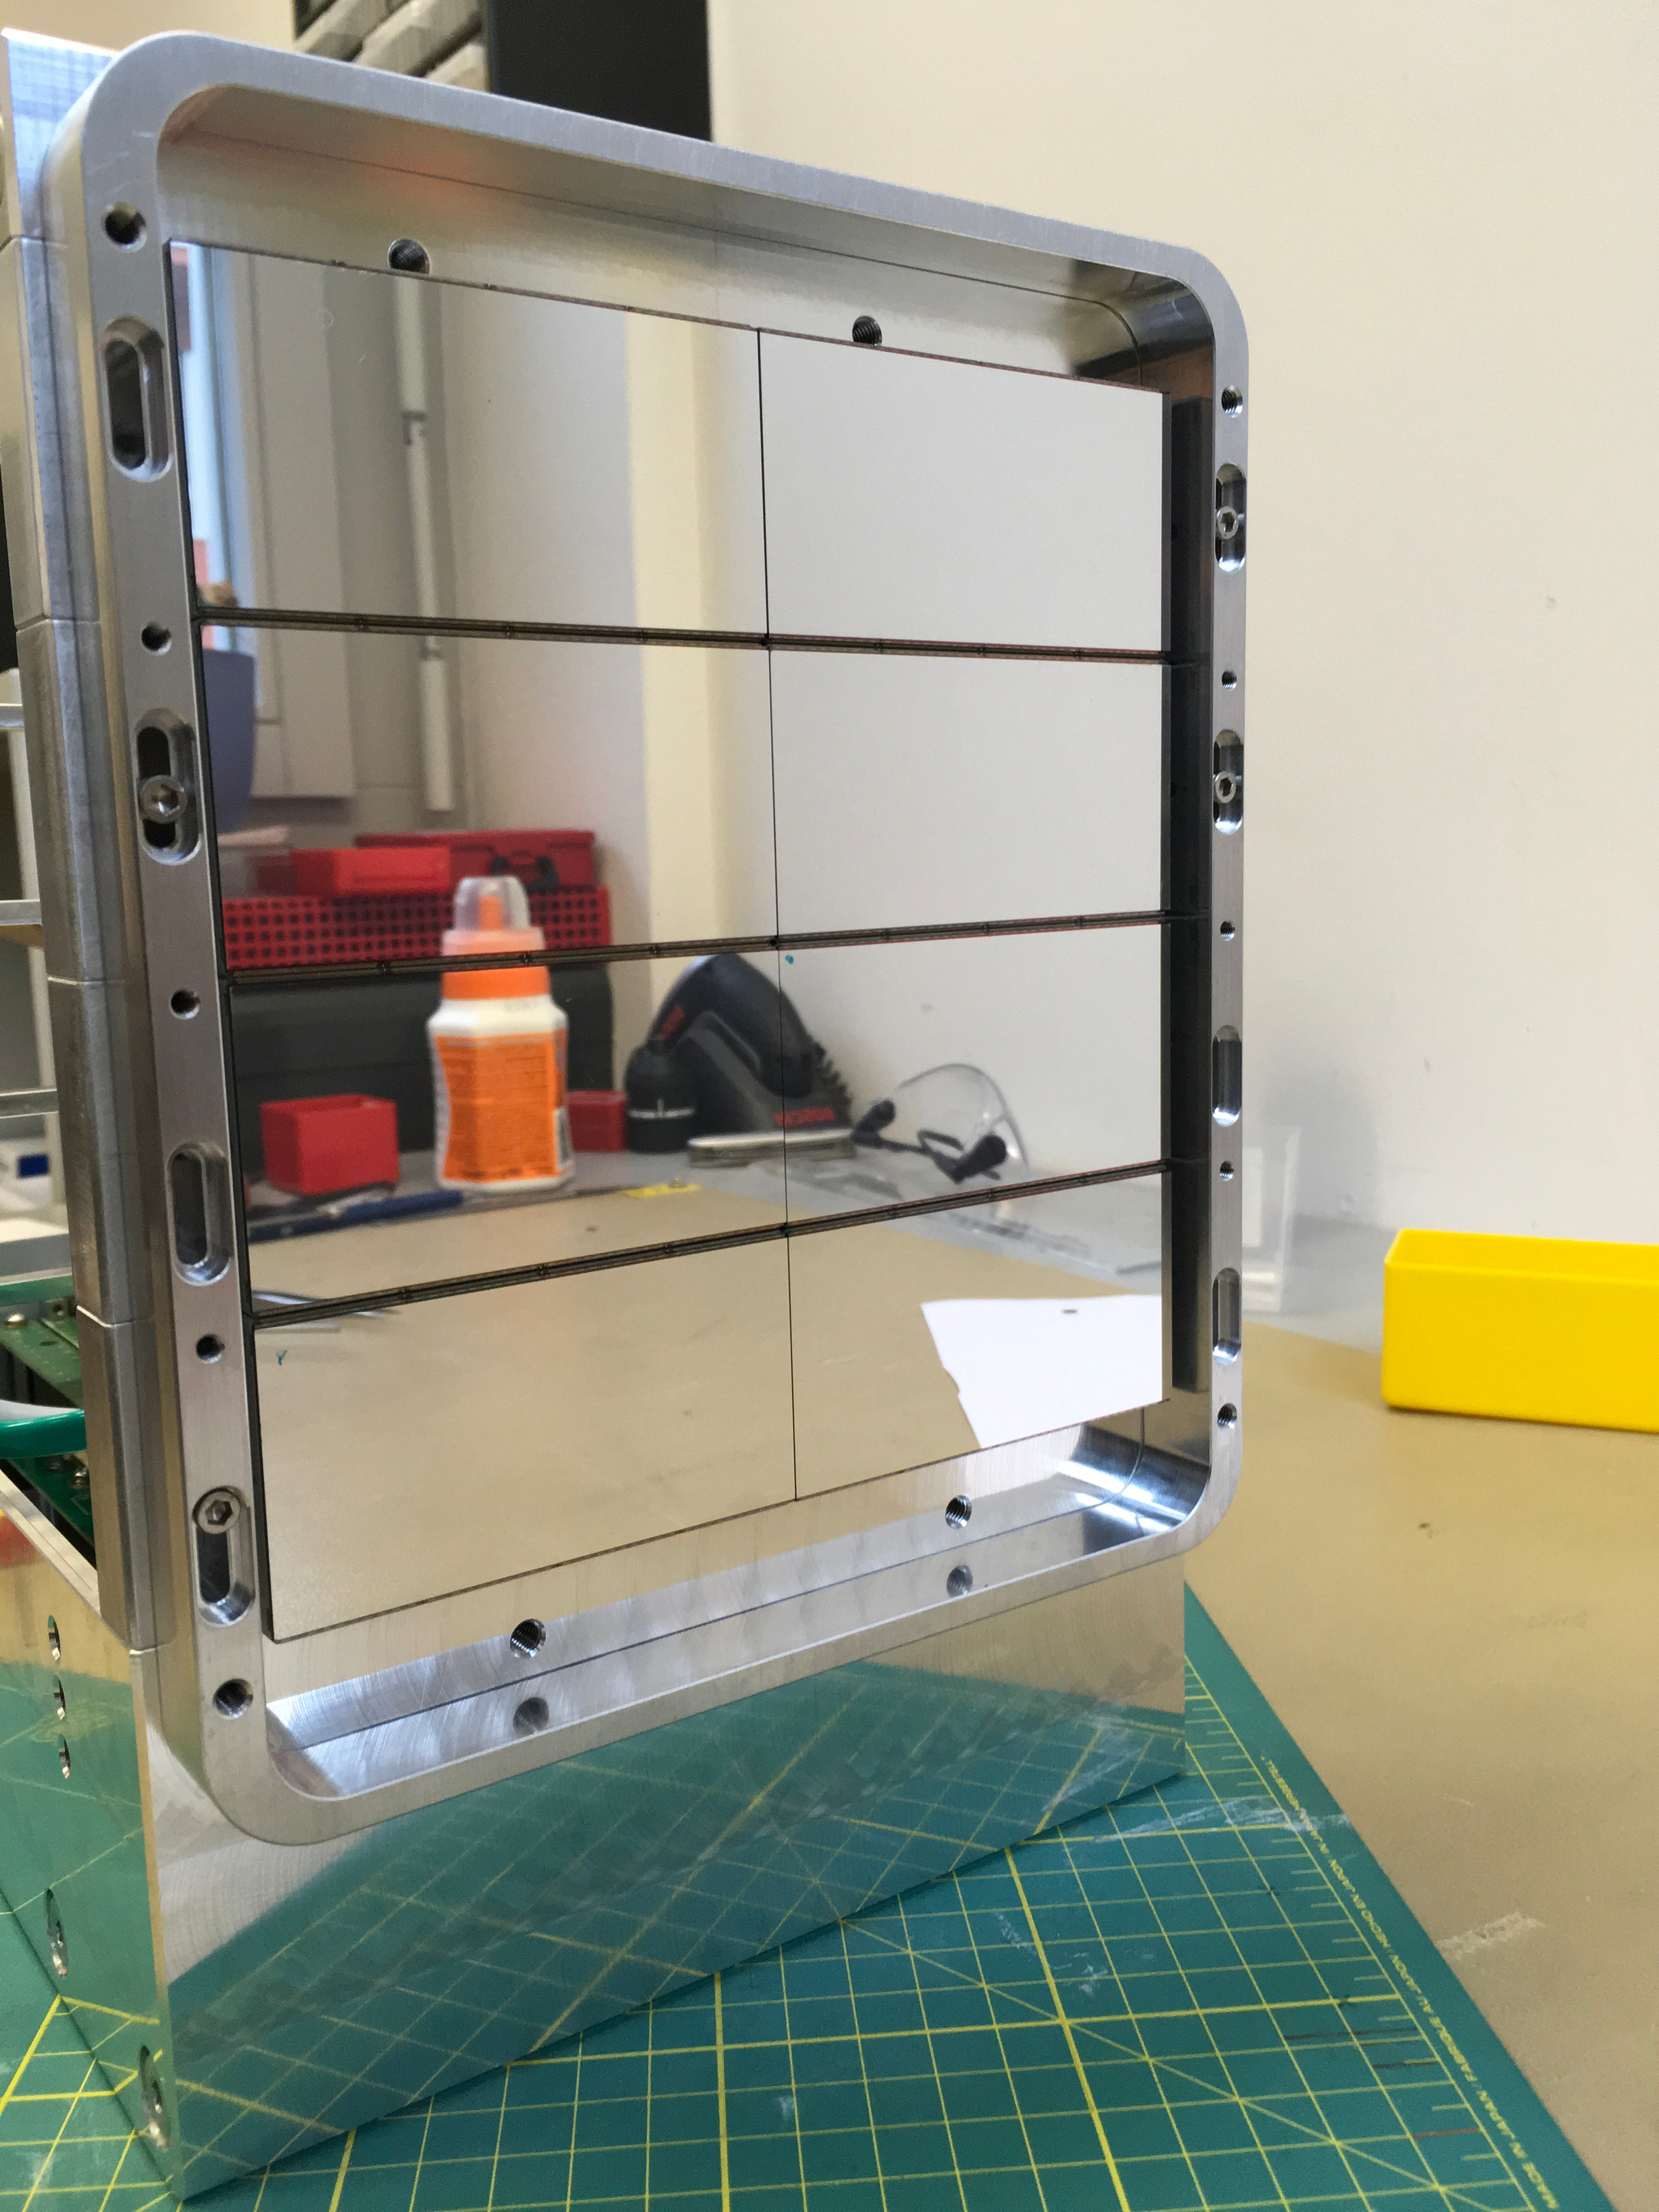
\includegraphics[width=0.30\textwidth]{jungfraudetector.jpg}
\caption{Jungfrau detector}
\label{fig:jfdetector}
\end{figure}


\subsection{Data processing algorithm (PSI)}
conversion from detector data to energy and number of photons\\

 summation of frames\\

 clustering (reference?)\\

\subsection{Alpaka implementation of fast data processing (Jonas, Florian)}


\subsection{Benchmark tests (Jonas, Florian)}
Design, objectives, and evaluation of tests

\section{Results}
\subsection{Achieved improvements (Jonas)}
Results of tests of software parts on various computing hardware using suitable Alpaka backends\\

Where are the bottlenecks\\

Available capacity on GPUs\\

Best system

\subsection{Experiences from practical application of improved code (PSI)}
Application results

\section{Conclusions and Outlook}

Is presented method applicable / useful for other detectors, e.g. AGIPD? \\

calculation on FPGAs in the future


\section{Acknowledges}
Thanks to Alpaka developers.....\\

This project has received funding from the European Union's Horizon 2020 research and innovation programme under grant agreement No 654220 (EUCALL).

\newpage

\begin{sloppypar}
\printbibliography
\end{sloppypar}
\end{document}
